% ==================================================
% Main Use Cases Description
% ==================================================
\section{Description of the Main Use Cases}

This section provides a detailed description of the main use cases of the proposed system. Each use case is presented through its actors, preconditions, nominal flow, as well as alternative and exceptional scenarios. In addition, system sequence diagrams are provided to illustrate the dynamic interactions between the user and the system.

% ==================================================
% UC01 -- Authentication
% ==================================================

\subsection{UC01 -- User Authentication (Login)}

\begin{table}[H]
	\centering
	\renewcommand{\arraystretch}{1.3}
	\begin{tabular}{|p{4cm}|p{10cm}|}
		\hline
		
		\textbf{Use Case Name} & Authentication \\ 
		\hline
		
		\textbf{Primary Actor} & User\\ 
		\hline
		
		\textbf{Preconditions} &
		\begin{itemize}
			\item The user has a valid account.
		\end{itemize} \\ 
		\hline
		
		\textbf{Nominal Sequence} &
		\begin{enumerate}
			\item The user accesses the login page.
			\item The system displays the authentication form.
			\item The user enters credentials and submits the form.
			\item The system validates the credentials.
			\item The system grants access and creates a session.
		\end{enumerate} \\ 
		\hline
		
		\textbf{Alternative Sequence} &
		\textbf{A1 -- Invalid input format}
		\begin{itemize}
			\item The system detects missing or incorrect data.
			\item The user is asked to correct the input.
		\end{itemize} \\ 
		\hline
		
		\textbf{Exceptional Sequence} &
		\textbf{E1 -- Incorrect credentials}
		\begin{itemize}
			\item The system declines authentication.
			\item An error message is displayed.
		\end{itemize} \\ 
		\hline
		
		\textbf{Postcondition} &
		The user is authenticated and redirected to the appropriate dashboard. \\ 
		\hline
		
	\end{tabular}
	\caption{Use Case Description -- User Authentication}
\end{table}

\begin{figure}[H]
	\hspace{-1.5cm}
	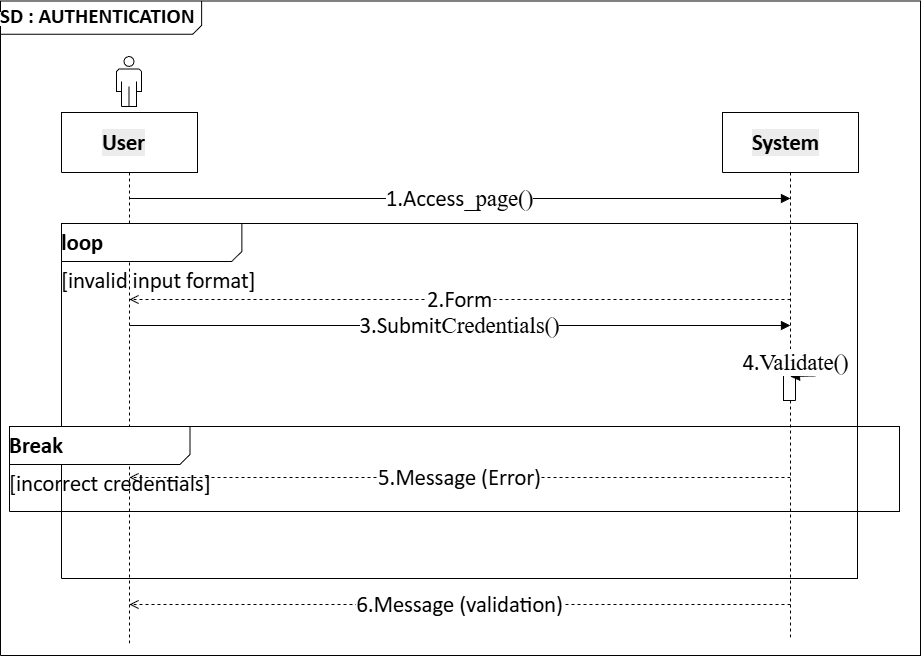
\includegraphics[width=1.15\textwidth]{images/diagrammes/Authentication}
	\caption{System Sequence Diagram -- UC01 Authentication}
\end{figure}


This diagram illustrates the interaction between the user and the system during the authentication process. The user initiates the process by entering credentials. The system then validates the provided information and responds either by granting access (successful authentication) or by displaying an error message in case of failure.

% ==================================================
% UC02
% ==================================================

\subsection{UC02 -- Decide Delivery Mission}

\begin{table}[H]
	\centering
	\renewcommand{\arraystretch}{1.3}
	\begin{tabular}{|p{4cm}|p{10cm}|}
		\hline
		
		\textbf{Use Case Name} & Decide Delivery Mission \\ 
		\hline
		
		\textbf{Primary Actor} & Transporter \\ 
		\hline
		
		\textbf{Objective} & Accept or reject a delivery mission. \\ 
		\hline
		
		\textbf{Preconditions} &
		\begin{itemize}
			\item The transporter is authenticated.
			\item A delivery request exists.
		\end{itemize} \\ 
		\hline
		
		\textbf{Nominal Sequence} &
		\begin{enumerate}
			\item The system sends a delivery request.
			\item The transporter views mission details.
			\item The transporter accepts the mission.
			\item The system records and updates the mission.
		\end{enumerate} \\ 
		\hline
		
		\textbf{Alternative Sequence} &
		\textbf{A1 -- Mission Rejected}
		\begin{itemize}
			\item The transporter rejects the mission.
			\item The system searches for another transporter.
		\end{itemize} \\ 
		\hline
		
		\textbf{Exceptional Sequence} & 
		\textbf{E1 -- No Transporter Available in Region}
		\begin{itemize}
			\item The system fails to find an available transporter within the specified geographical region.
			\item The system flags the mission status as pending.
		\end{itemize} \\ 
		\hline
		
		\textbf{Postcondition} &
		The mission is assigned if accepted. \\ 
		\hline
		
	\end{tabular}
	\caption{Use Case Description -- Decide Delivery Mission}
\end{table}

\begin{figure}[H]
	\hspace{-1.5cm}
	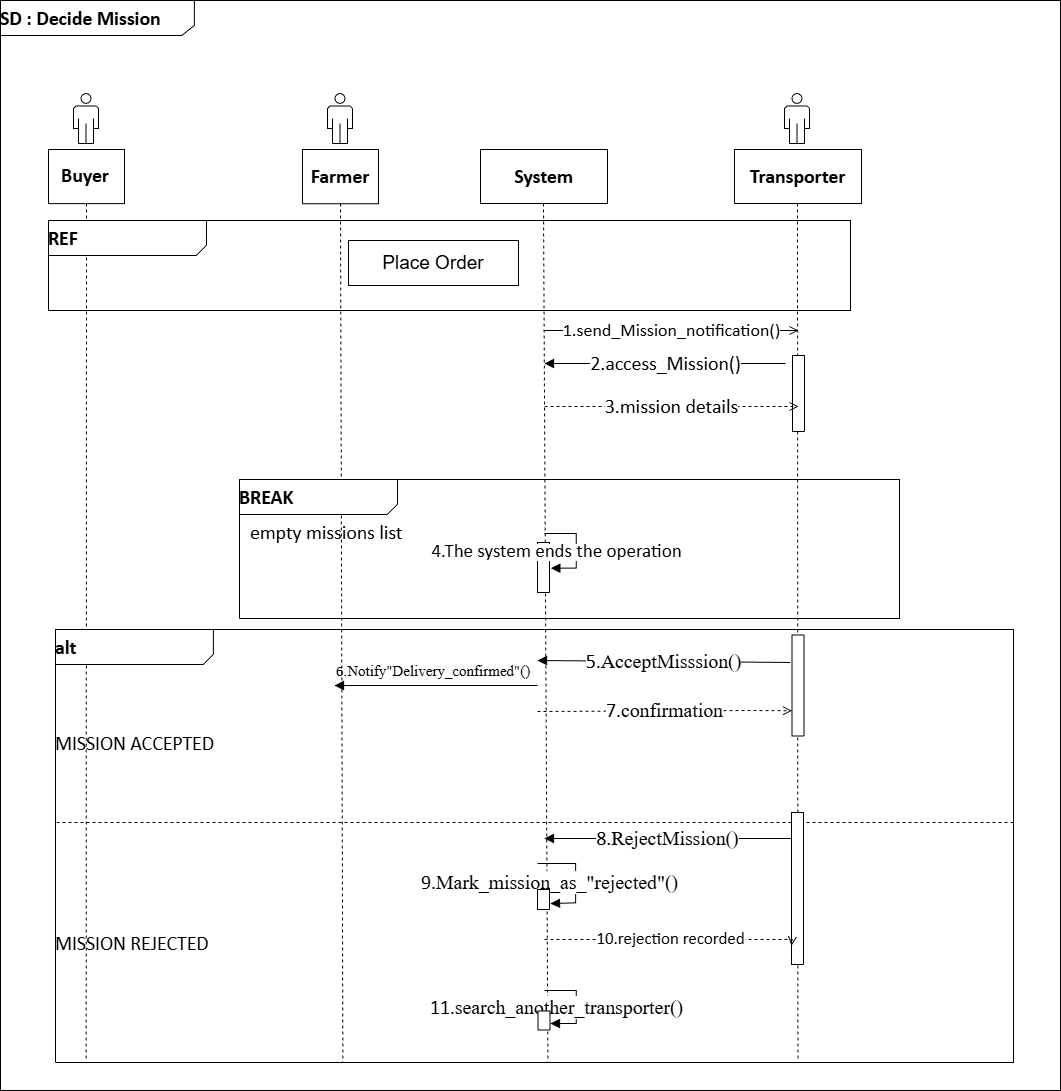
\includegraphics[width=1.15\textwidth]{images/diagrammes/DecideMilestone}
	\caption{System Sequence Diagram -- Decide Delivery Mission}
\end{figure}

 
This diagram shows how the system interacts with the transporter when a delivery request is issued. The system sends a notification, and the transporter evaluates the mission details before making a decision. Based on this decision, the system updates the mission status and notifies the relevant actors.

% ==================================================
% UC03
% ==================================================

\subsection{UC03 -- User Validation}

\begin{table}[H]
	\centering
	\renewcommand{\arraystretch}{1.3}
	\begin{tabular}{|p{4cm}|p{10cm}|}
		\hline
		
		\textbf{Use Case Name} & User Validation \\ 
		\hline
		
		\textbf{Primary Actor} & Ministry Administrator \\ 
		\hline
		
		\textbf{Objective} & Approve or reject user registration. \\ 
		\hline
		
		\textbf{Preconditions} & Authentication \\ 
		\hline
		
		\textbf{Nominal Sequence} &
		\begin{enumerate}
			\item The user submits a registration request.
			\item The system stores the request.
			\item The administrator reviews the information.
			\item The administrator approves the request.
			\item The system notifies the user.
		\end{enumerate} \\ 
		\hline
		
		\textbf{Alternative Sequence} & 
		\textbf{A1 -- Documents Unclear}
		\begin{itemize}
			
			\item The system requests the user to re-submit clearer information or higher-quality documents.
			\item The registration request remains in a pending status until the user updates it.
		\end{itemize} \\ 
		\hline
		
		\textbf{Exceptional Sequence} &
		\textbf{E1 -- Invalid documents}
		\begin{itemize}
			\item The request is rejected.
			\item The user is notified.
		\end{itemize} \\ 
		\hline
		
		\textbf{Postcondition} &
		The account is activated. \\ 
		\hline
		
	\end{tabular}
	\caption{Use Case Description -- User Validation}
\end{table}

\begin{figure}[H]
	\hspace{-1.5cm}
	\includegraphics[width=1.15\textwidth]{images/diagrammes/userValidation}
	\caption{System Sequence Diagram -- User Validation}
\end{figure}

 
This diagram represents the validation process handled by the administrator. After a registration request is submitted, the system stores it and allows the administrator to review it. The final decision (approval or rejection) is then communicated to the user.

% ==================================================
% UC04
% ==================================================

\subsection{UC04 -- Search Product}

\begin{table}[H]
	\centering
	\renewcommand{\arraystretch}{1.3}
	\begin{tabular}{|p{4cm}|p{10cm}|}
		\hline
		
		\textbf{Use Case Name} & Search Product \\ 
		\hline
		
		\textbf{Primary Actor} & Buyer \\ 
		\hline
		
		\textbf{Objective} & Search for available products. \\ 
		\hline
		
		\textbf{Preconditions} & \begin{itemize}
			\item The user is authenticated.
		\end{itemize}  \\ 
		\hline
		
		\textbf{Nominal Sequence} &
		\begin{enumerate}
			\item The user enters a keyword in the search bar.
			\item The system processes the request.
			\item The system displays matching products.
		\end{enumerate} \\ 
		\hline
		
		\textbf{Alternative Sequence} & 
		\textbf{A1 -- Filtered Search}
		\begin{itemize}
			\item The user applies specific search filters (e.g., category, price range, region, or availability).
			\item The system refines the search query based on the selected parameters.
			\item The system displays the filtered list of products matching the criteria.
		\end{itemize} \\ 
		\hline
		
		\textbf{Exceptional Sequence} &
		\textbf{E1 -- No results found}
		\begin{itemize}
			\item The system displays a "No products match your search" message.
			\item The system suggests alternative keywords or prompts the user to clear applied filters.
		\end{itemize} \\ 
		\hline
		
		\textbf{Postcondition} &
		A list of products matching the user's search or filter criteria is displayed. \\ 
		\hline
		
	\end{tabular}
	\caption{Use Case Description -- Search Product}
\end{table}

\begin{figure}[H]
	\centering
	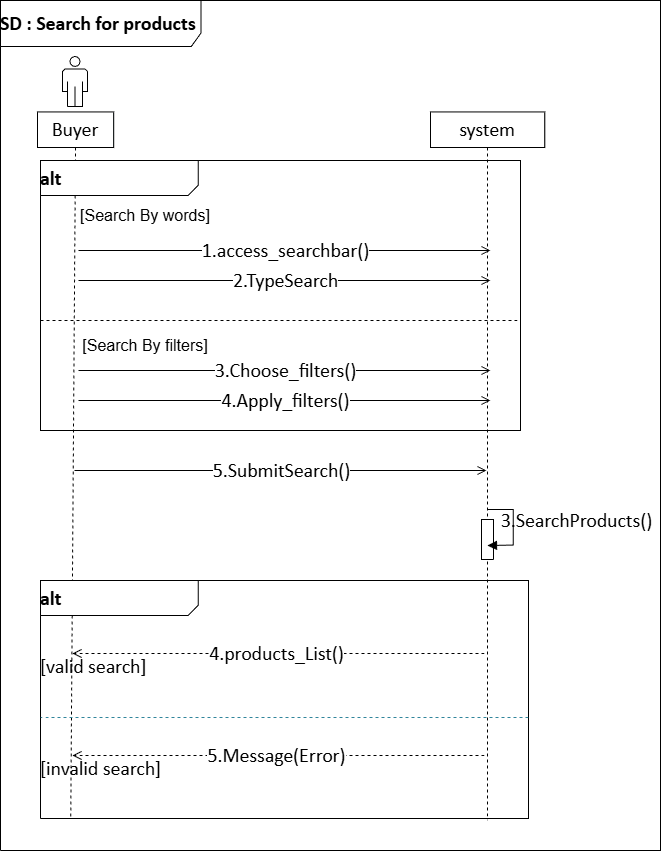
\includegraphics[width=0.95\textwidth]{images/diagrammes/SearchProduct}
	\caption{System Sequence Diagram -- Search Product}
\end{figure}

This diagram illustrates how the buyer interacts with the system to search for products. The user submits a query, and the system processes it to retrieve and display relevant results. If no products match the query, an appropriate message is returned.

% ==================================================
% UC05
% ==================================================

\subsection{UC05 -- Decide Order}

\begin{table}[H]
	\centering
	\renewcommand{\arraystretch}{1.3}
	\begin{tabular}{|p{4cm}|p{10cm}|}
		\hline
		
		\textbf{Use Case Name} & Decide Order \\ 
		\hline
		
		\textbf{Primary Actor} & Farmer \\ 
		\hline
		
		\textbf{Objective} & Accept or refuse an order. \\ 
		\hline
		
		\textbf{Preconditions} & The farmer is authenticated \\ 
		\hline
		
		\textbf{Nominal Sequence} &
		\begin{enumerate}
			\item The farmer views pending orders.
			\item The farmer selects an order.
			\item The farmer accepts the order.
			\item The system updates the status.
		\end{enumerate} \\ 
		\hline
		
		\textbf{Alternative Sequence} &
		\textbf{A1 -- Order Refused}
		\begin{itemize}
			\item The farmer refuses the order.
			\item The system updates the status.
		\end{itemize} \\ 
		\hline
		
		\textbf{Exceptional Sequence} & 
		\textbf{E1 -- No Pending Orders Found}
		\begin{itemize}
			
			\item The system displays an empty state message (e.g., "No pending orders available") and the use case terminates.
		\end{itemize} \\ 
		\hline
		
		\textbf{Postcondition} &
		The order status is updated. \\ 
		\hline
		
	\end{tabular}
	\caption{Use Case Description -- Decide Order}
\end{table}

\begin{figure}[H]
	\centering
	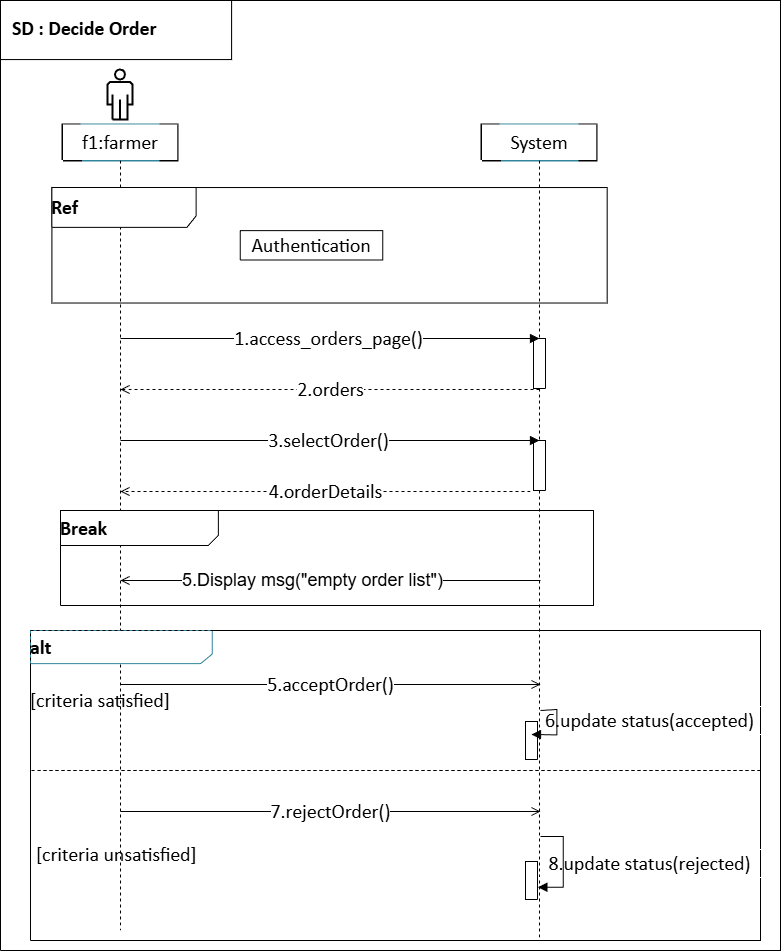
\includegraphics[width=0.95\textwidth]{images/diagrammes/decideOrder}
	\caption{System Sequence Diagram -- Decide Order}
\end{figure}

This diagram shows the interaction between the farmer and the system when handling orders. The farmer reviews order details and makes a decision. The system then records this decision and updates the order status accordingly.